\section{Crypto Recap}
\subsection{Objectives:}
\begin{itemize}
  \item{\textbf{Confidentiality}}
  \item{\textbf{Integrity}}
  \item{\textbf{Authenticity}}
  \item{\textbf{Availability}}
  \item{Authorization}
  \item{Non-Repudiation, Accountability}
  \item{Freshness}
  \item{Anonymity, Unlinkability}
  \item{Intervenability, Contro}
  \item{Transparency}
\end{itemize}

\subsection{Confidentiality-Encryption}
\subsubsection{Symmetric Ciphers}
\begin{itemize}
  \item Secret key for en- and decryption
  \item Much more efficient
  \item \textbf{Block cipher: }encryps a plaintext block of fixed len e.g.: \textit{Advanced Encryption Standard (AES)}
  \item \textbf{Stream cipher: }encrypts a bitstream e.g.:\textit{ChaCha20}
\end{itemize}

\subsubsection{Asymmetric Ciphers}
\begin{itemize}
  \item Public key for encryption
  \item Private key for decryption
  \item Ex.: RSA-based encryption
\end{itemize}

\subsection{Integrity, Authenticity-Signatures, MACs}
\subsubsection{MACs}
\begin{itemize}
  \item Symmetric cryptography
  \item Protects data integrity \& authenticity
  \item Ex.: Hash-based MAC
\end{itemize}

\subsubsection{Digital Signatures}
\begin{itemize}
  \item Asymmetric cryptography
    \begin{itemize}
      \item{\textbf{Signing with} private key}
    \end{itemize}
  \item{Protects data integrity \& authenticity}
  \item{Provices non-repudation}
\end{itemize}

\subsection{Block Cipher Modes of Operation}
\subsubsection{Electronic Code Book (ECB)}
\begin{itemize}
  \item{Each plaintext block is encrypted seperatly}
  \item{Inherintly insecure! -> Smae block = Same cipher}
\end{itemize}

\subsubsection{Cipher Block Chainning (CBC)}
\begin{itemize}
  \item Plaintext is chained to previous ciphertext by XOR and encrypted afterwards
  \item Difficult to apply securely -> implementations often vulnerable
\end{itemize}

\subsubsection{Galois Counter Mode (GCM)}
\begin{center}
  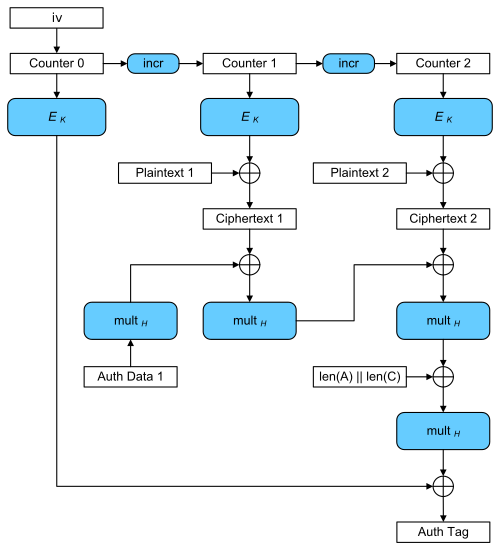
\includegraphics[width=0.5\columnwidth]{Resources/GCM-Galois_Counter_Mode_with_IV.svg.png}
\end{center}

\section{Tranport Layer Security (TLS)}
\subsection{TLS handshake protocol}
\begin{itemize}
  \item Parameter Negotiation
  \item Key exchange
  \item Authentication
\end{itemize}
\subsection{TLS record protocol}
\begin{itemize}
  \item Protection of integrity, authenticiy and confidentiality
  \item \textbf{Symmetric Cryptography:} e.g., block cipher, usually AES
\end{itemize}

\subsection{Attacks}
\begin{itemize}
  \item Attacks on the record layer
  \item Attacks on the session key
  \item Attacks on the private server key
    \begin{itemize}
      \item Attacks on implmentations: Timing Attacks, Heratbleed, Invalid Point Attacks
    \end{itemize}
  \item Attacks on TLs eco system
    \begin{itemize}
      \item Attacks on certificates and the PKI
      \item Attacks on the browser GUI
    \end{itemize}
\end{itemize}

\subsection{Overview TLS 1.0-1.2 \& TLS 1.3}
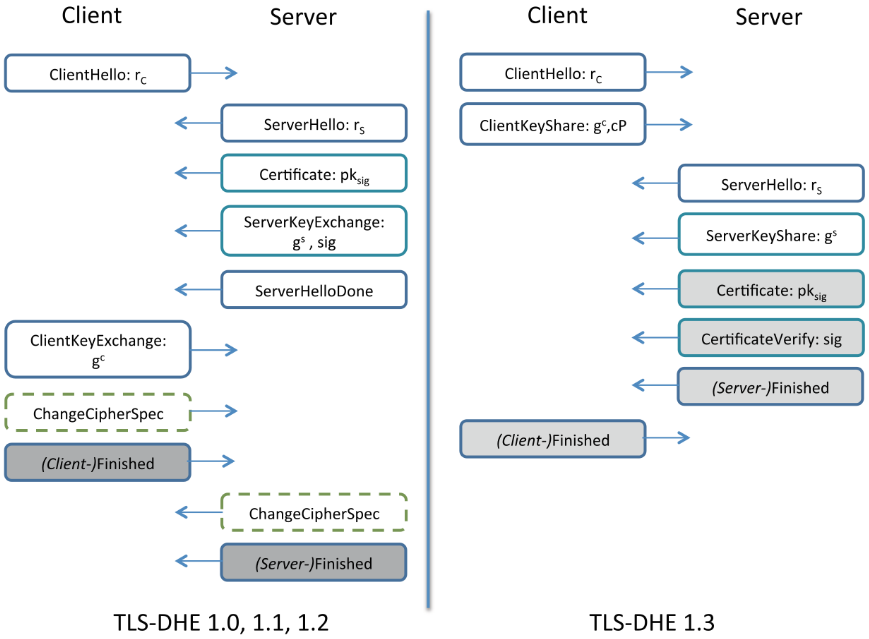
\includegraphics[width=0.8\columnwidth]{Resources/tls.png}

\subsection{HKDF Key Derivation Function}

\subsection{Forward Secrecy}
\begin{itemize}
  \item TLS 1.3 using certificate-based Authentification: \textbf{forward secrecy}
  \item TLS 1.3 using pre-shared keys (PSK):
    \begin{itemize}
      \item PSK using \textit{elliptic-curve} Diffie-Hellman: \textbf{forward secrecy}
      \item PSK without EC-DHE (symmetric-only) and zero-round-trip data: \textbf{no forward secrecy}
    \end{itemize}
\end{itemize}

\subsection{Datagramm TLS}
\begin{itemize}
  \item DTLS is identical to TLS where possible
  \item DTLS has to introcue new mechanisms
    \begin{itemize}
      \item Explicit sequence numbers
      \item Retransmission timer for handshake message
      \item Message re-ordering for the handshake
      \item Fragmentation of large handshake messages into serveral DTLS records
      \item Optional replay detection
      \item Invalid records are discarded (silently)
      \item Denial-of-Service countermeasures: statless cookies, HelloRetryRequest
    \end{itemize}
\end{itemize}

\section{Network Layer Security: IPsec}
\subsection{TLS limitations}
\begin{itemize}
  \item Does not protect all traffic between hosts
    \begin{itemize}
      \item Protects only a single connection; new connection => new key agreement or session resumption necessary
      \item Non-TCP traffic (resp. non-UDP trafic for DTLS) cannto be protected
    \end{itemize}
  \item Does not protect the TCP layer (RST attacks on TCP are possible which terminate TLS connection)
  \item Application specific: applications have to be modified to use TLS/DTLS
  \item Using a TLS-based tunel for VPNs has disadvangates (TCP) (DTLS good option tho)
\end{itemize}

\subsection{Overview IPsec}
\begin{itemize}
  \item Goal: Protect IP packets cryptographically
    \begin{itemize}
      \item Confidentiality
      \item Integrity \& Authenticity
    \end{itemize}
  \item Seperation of packet protection from key exchange
    \begin{itemize}
      \item Protocols for packet encryption and authentification:
        symmetric crypto, implemented in the TCP/IP stack
      \item Key Exchange completly unrelated:
        asymmetric (+symmetric) crypto, implemented as network daemon
    \end{itemize}
\end{itemize}
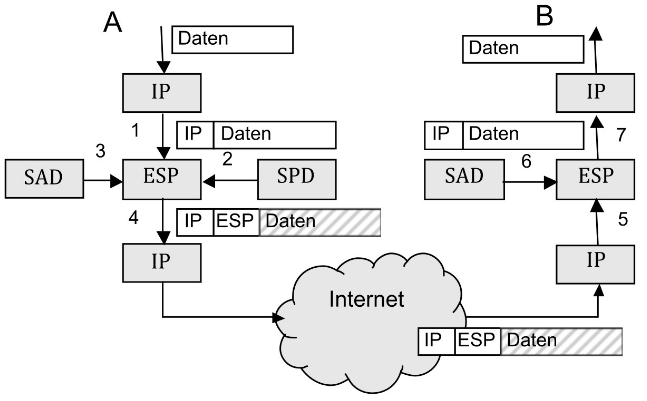
\includegraphics[width=\columnwidth]{Resources/ipsec_overview.png}

\subsection{Packet Formats and Operational Modes}
\subsubsection{Authentification Header (AH)}
\begin{itemize}
  \item Integrity \& Authenticity only
  \item Partially protects "outer" IP header
    \begin{itemize}
      \item Variable fields cannot be includes
        \begin{itemize}
          \item Flags, Fragment Offset, TTL, Header Checksume
        \end{itemize}
      \item Other fields are included in MAC computation
        \begin{itemize}
          \item Version, IP header length, total length, identification, Protocol (must be AH), source/dest Address
        \end{itemize}
    \end{itemize}
\end{itemize}
\subsubsection{Encapsulating Security Payload (ESP)}
\begin{itemize}
  \item Confidentiality, Integrity \& Authenticity
  \item Does not protect "outer" IP header
\end{itemize}
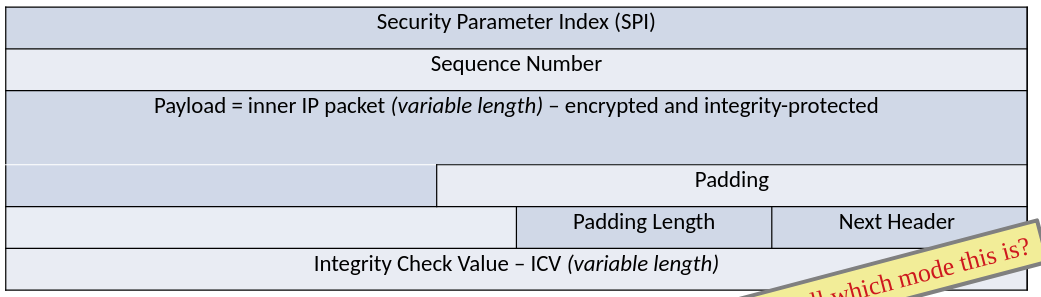
\includegraphics[width=\columnwidth]{Resources/esp.png}
\begin{itemize}
  \item SPI: SA-Identifier
  \item Next Header: type of payload data (e.g. IPV4)
  \item Integrity Check Value: data for authentification / integrity protection
    \begin{itemize}
      \item Message Authentification Code (MAC)
    \end{itemize}
  \item SAs are negotiated in the key exchange
  \item Sender side: Packet must be categorized to determine which SA applies (By parameters such as destination=)
  \item Receiver side: Determines SA from IPsec header of received packet
  \item SA Parameters:
    \begin{itemize}
      \item IPsec protocol (AH or ESP)
      \item Authentification alrogrithm and key
      \item Encryption algorithm and key
      \item IPsec mode (transport or tunnel)
      \item SA lifetimne
      \item Sequence number: current counter
      \item On reciver side: "Sliding Window" for replay protection
    \end{itemize}
\end{itemize}

\subsection{Scenarios}
\begin{itemize}
  \item Host to host
  \item Host to gateway
  \item Gateway to gateway
\end{itemize}

\subsection{The Internet Key Exchange (IKE)}
\begin{itemize}
  \item So far, keys are already exchanges, SAs negotiated... but how?
  \item Authentification of the communication endpoints
  \item Dynamic negotiation fo algorithms and parameters
  \item Key establishment
    \begin{itemize}
      \item Forward Secrecy
    \end{itemize}
  \item Resistance to DoW attacks
  \item Efficiency (computation, messages, round trips)
\end{itemize}

\subsection{IKEv1}
\begin{itemize}
  \item Phase 1: main mode vs. aggressive mode
  \item Authentification modes:
    \begin{itemize}
      \item Digital Signatures
      \item Public key encryption(PKE): two variants (rarely used)
      \item Pre-shared keys(PSK)
    \end{itemize}
  \item Phase 2 (quick mode)
    \begin{itemize}
      \item With DH (=> forward secrecy)
      \item Without DH (=> no forward secrecy)
    \end{itemize}
\end{itemize}
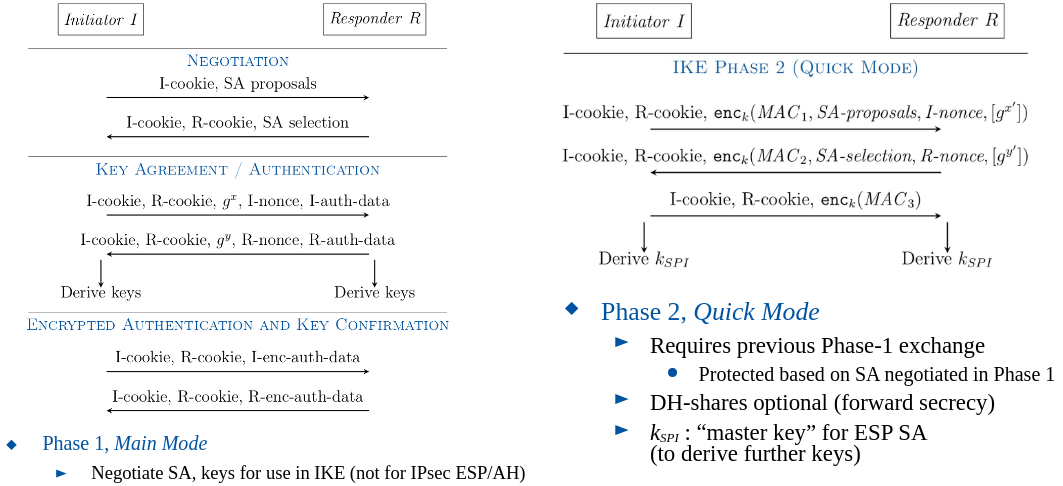
\includegraphics[width=\columnwidth]{Resources/ikev1.png}

\subsubsection{Discussion}
\begin{itemize}
  \item Complicated
    \begin{itemize}
      \item Information from serveral (complex) RFCs required
      \item Many options variants
    \end{itemize}
  \item Gneric
    \begin{itemize}
      \item Clean seperation of different phases and functionalities
        \begin{itemize}
          \item Can be advantagous in theory, but leads to inefficincies
        \end{itemize}
      \item Intended as general handshake and key agreement protocol, not only for IPsec
        \begin{itemize}
          \item In practice: only used for IPsec
        \end{itemize}
      \item Inneficient
        \begin{itemize}
          \item Requires too many round trips
        \end{itemize}
      \item Inadequate DoS protection
        \begin{itemize}
          \item IKEv1 uses stateful cookies
        \end{itemize}
    \end{itemize}
\end{itemize}

\subsection{IKEv2}
\begin{itemize}
  \item Phase 2 (partially) combindes with Phase 1
    \begin{itemize}
      \item More efficient thatn IKEv1
      \item Initial negotiation of IPsec SA included
    \end{itemize}
  \item Additional SAs can be negotiaded in furhter Phase 2 protocol runs
  \item Simplified specification
    \begin{itemize}
      \item Essential information in one RFC
      \item No distinction main mode vs. aggressive mode
    \end{itemize}
  \item DoS protection using statless cookies: optional
\end{itemize}
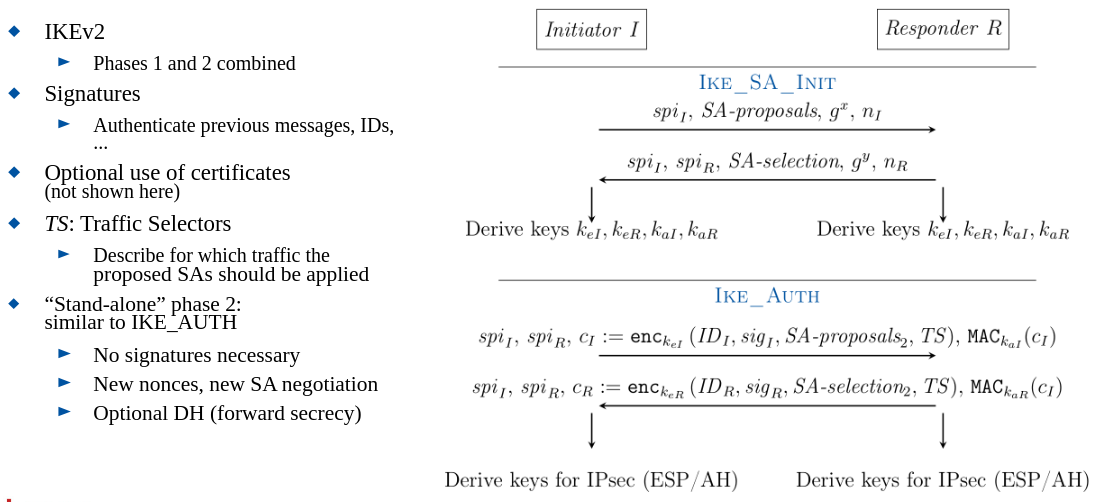
\includegraphics[width=\columnwidth]{Resources/ikev2.png}

\subsection{SA Proposals}
\begin{itemize}
  \item Serverl proposals possible
  \item Proposal contains transforms
  \item Differnten options for each transform possible
    \begin{itemize}
      \item Exactly one transform has to be selected
    \end{itemize}
\end{itemize}
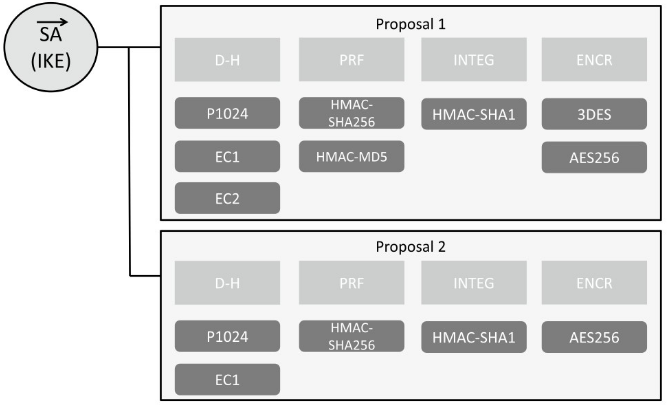
\includegraphics[width=0.7\columnwidth]{Resources/ike_sa_proposal.png}

\section{Security on Layer 2 (MAC Layer, Ethernet)}
\subsection{Attacks}
\begin{itemize}
  \item MAC address spoofing
  \item ARP spoofing
  \item ARP cache poisoning
\end{itemize}

\subsection{Network Access Control}
\begin{itemize}
  \item \textbf{Frontend} protocols: Cient -> Network Access Server
    \begin{itemize}
      \item Point-to-Point connections: PPP
      \item LAN: PPPoE, EAPoL
      \item WLAN: WPA/WPA2/WPA3, EAPoL
    \end{itemize}
  \item \textbf{Backend} protocols: Network Access Server --> Authentication Server AAA protocols (Authentication, Authorization, Accounting)
    \begin{itemize}
      \item Radius, Diameter
      \item TACACS+
    \end{itemize}
\end{itemize}
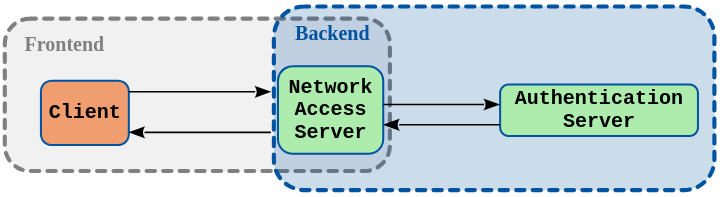
\includegraphics[width=0.6\columnwidth]{Resources/network_access_control.png}

\subsubsection{Radius - Remote Authentification Dial-In User Service}
\begin{itemize}
  \item Backend protocol
  \item Dial-In Server
    \begin{itemize}
      \item E.g. DSL
      \item Company infrastructure
    \end{itemize}
\end{itemize}
\textbf{Packet Format}\\
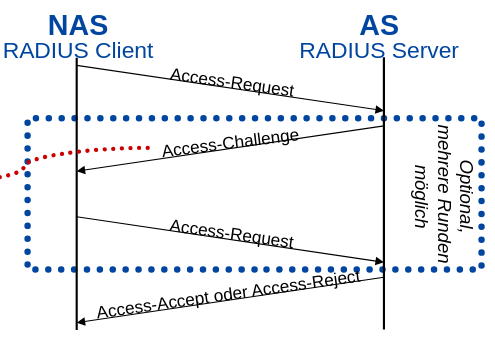
\includegraphics[width=0.7\columnwidth]{Resources/radius.png}
\textbf{Security}\\
\begin{itemize}
  \item Old protocol
    \begin{itemize}
      \item Tries to protect sesitive data only
      \item Insecure cryptography
    \end{itemize}
  \item Uses only over secure protocols
    \begin{itemize}
      \item Usually TLS
    \end{itemize}
  \item RADIUS successor: Diameter
    \begin{itemize}
      \item Fmore flexible, extensible, application-aware
      \item "Security" features removed, no more insecure crypto of RADIUS
        => To be used over secure protocols TLS/DTLS/IPsec
    \end{itemize}
\end{itemize}

\subsubsection{Point-to-Point Protocol (PPP)}
\begin{itemize}
  \item \textbf{PPP: }Frontend protocol to connect two devices
    \begin{itemize}
      \item Typically used for dial-up connections (e.g. DSL)
      \item Transported over Layer 2 protocol (e.g. ethernet)
    \end{itemize}
  \item Authentification mechanisms
    \begin{itemize}
      \item PAP: username/password
      \item CHAP: Challange Handshake Authentification Protocol
      \item EAP: Extensible Authentification Protocol
    \end{itemize}
  \item \textbf{PPPoE: }PPP over Ethernet (e.g. used for DSL connections)
    \begin{itemize}
      \item Discovery: Client negotiates session with network access server
      \item PPP Session: PPP frames are encapsulated in ethernet frames; potentially several hops
    \end{itemize}
\end{itemize}

\subsubsection{Extensible Authentification Protocol (EAP)}
\begin{itemize}
  \item Extensible authentification framework
    \begin{itemize}
      \item Fronted protocol for lcient authentification
      \item Server send request (e.g. challenge, ident. request, ..)
      \item Client responds
      \item Server sends success or failure message
      \item EAP messages can be transported in RADIUS messages (as RADIUS attribute) for backend communication
    \end{itemize}
  \item EAPoL: EAP over LAN
\end{itemize}

\subsubsection{Port Based Network Access Control (PNAC)}
\begin{itemize}
  \item Authentification of clients befre they can use the network (LAN)
    \begin{itemize}
      \item Client connect to the network
        \begin{itemize}
          \item Authentification traffic is allowed
        \end{itemize}
      \item Switch port can only be used for other purposes after successful authentification
      \item Re-authentification after timeouts, link-down, etc.
    \end{itemize}
  \item PNAC uses EAPoL
  \item Terminology: Port Access Entities (PAE)
    \begin{itemize}
      \item Client: supplicant
      \item Netowrk access server: authenticator
      \item Attention: "port"
    \end{itemize}
\end{itemize}

\subsection{MACsec}
\begin{itemize}
  \item cryptographically protect the ethernet layer
  \item Based on MACsec Key Agreeement (MKA)
    \begin{itemize}
      \item After successful authentification (typically EAP)
      \item Derives key from CAK - connectivity association key (pre-shared)
      \item Key can be set up by EAP (e.g. EAP-TLS)
    \end{itemize}
\end{itemize}
 \subsubsection{Frame}
 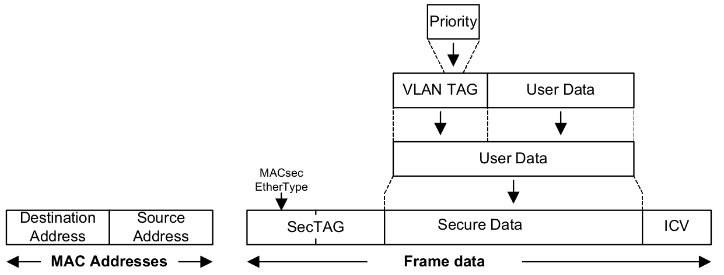
\includegraphics[width=0.8\columnwidth]{Resources/macsec_frame.png}
 \begin{itemize}
  \item Data cen be encryped and/or authentificated
  \item AES-GCM is supported
 \end{itemize}
 \textbf{Security TAG (SecTAG)}\\
 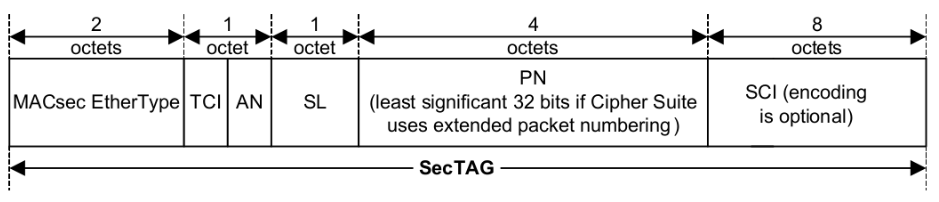
\includegraphics[width=0.8\columnwidth]{Resources/sec_tag.png}
 \begin{itemize}
  \item TCI: TAG Control Information
  \item AN: Association Number
  \item SL: Short Length (payload length; for short frames only)
  \item PN: Packet Number
  \item SCI: Secre Channel Identifier (edentify SA, when CA needs ore than 4)
    \begin{itemize}
      \item SA is identified by SCI (optional) and AN
    \end{itemize}
 \end{itemize}
 \subsection{Summary}
\begin{itemize}
  \item Security on Layer 2 can protect all higher Layer
    \begin{itemize}
      \item But: only in same network
      \item Does nt work accross Layer 3 routers
    \end{itemize}
  \item Network Access Control protects access to the network
    \begin{itemize}
      \item Client Authentification
      \item RADIUS/DIAMETER
      \item EAP
      \item Port-Based Access Control
    \end{itemize}
  \item MACsec protects traffic
  \begin{itemize}
    \item Encryption \& authentification
  \end{itemize}
\end{itemize}

\section{Wireless Security}
\subsection{WiFi Security}
\subsubsection{Historic Overview}
\begin{itemize}
  \item 1999: WEP (Wired Equivilaent Privacy)
    \begin{itemize}
      \item Goal: "as secure as a wired LAN"
      \item Insecure, various attacks known
    \end{itemize}
  \item 2003: WPA (WiFi Protected Access)
    \begin{itemize}
      \item Improved protocols; most known attacks on WEP prevented
      \item Enterprice Mode
      \item But: Requirement ofr hardware-compatibility with WEP devices => Encryption improved, but still based on obsolete stream cipher
    \end{itemize}
  \item 2004: WPA2 (still used) 
    \begin{itemize}
      \item Similar to WPA, but AES-based encryption: AES-CCMP
    \end{itemize}
  \item 2018: WPA3 (supported by new devices) 
    \begin{itemize}
      \item Serveral improvements: 
        Prevention of offline-attacks on pre-shared keys, forward secrecy, encryption for "open" WLANs
    \end{itemize}
\end{itemize}
\subsubsection{WPA/WPA2 Security}
\begin{itemize}
  \item Personal Mode
    \begin{itemize}
      \item Pre-Shared Keys
    \end{itemize}
  \item Enterprise Mode 
    \begin{itemize}
      \item EAP-TLS, PEAP, EAP-TTLS
    \end{itemize}

\textbf{AES-CCMP}\\
  \item Authenticated Encryption with Associated Data (AED)
  \item AES-CCM
    \begin{itemize}
      \item Authentication: CBC-MAC
      \item Encryption: Counter Mode (CTR)
      \item MAC and encyprion: computed simultaneously
    \end{itemize}
\end{itemize}

\textbf{4-Way Handshake}\\
\begin{itemize}
  \item Based on Pairwise Master Key (PMK)
    \begin{itemize}
      \item Personal Mode (WPA-PSK):
        Computed from passphrase and SSID (as "salt") using PBKDF2 (password-based key derivation function)
      \item Enterprise Mode: Established by key exchange protocol (e.g. EAP-TLS, PEAP)
    \end{itemize}
  \item 4-Way HS to derive Pairwise Transient Key (PTK) 
    \begin{itemize}
      \item Exchance nonces
      \item PTK is derived by hashing PMK, nonces, MAC addrs 
      \item Furhter key (for differnet purposes) derived from PTK 
      \item Client gets Group Temporary Key from AP (encrypted) 
      \item Message Integrity Code(MIC): MACs for integrity protection, key confirmation 
    \end{itemize}
  \item KRACK (2018): Key reinstallation attacks => meanwhile prevented by software/firmware updates 
  \item Problem: Offline attacks against passphrase 
\end{itemize}

\subsubsection{WPA 3 Improvements}
\begin{itemize}
  \item Mandatory Protected Managment Frames
    \begin{itemize}
      \item Prevents deauthentication attacks (DoS)
    \end{itemize}
  \item Replace PSK Authentication with SAW protocol 
    \begin{itemize}
      \item Simultaneous Authentication among Equals (SAE):
        "Dragonfly" handshake
      \item Prevents offline attacks on passphrase 
      \item Based on elliptic curve cryptography by default
    \end{itemize}
  \item Forward Secrecy based on Diffie-Hellman 
  \item 192-bit Security Mode (optional) 
    \begin{itemize}
      \item AES-256 (GCM)
      \item SHA-384 
      \item 284-bit elliptic curves or RSA with at least 3K bits 
    \end{itemize}
\end{itemize}

\subsubsection{Simultaneous Authentication among Equals}
\begin{itemize}
  \item SAE "Dragonfly" authenicates participants and establishes PMK
    \begin{itemize}
      \item Based on passphrase and (EC-)Diffie-Hellman
      \item Can be initiated simultaneously by both parties (useful for mesh networking) 
    \end{itemize}
  \item 4-Way Handshake 
    \begin{itemize}
      \item Esablishes PTK basen on PMK
      \item Same as in WPA2 
      \item But now: PMK with much higher entropy => Offlione attacks not practical 
    \end{itemize}
  \item Hash-to-Group: "Hunting and Pecking" 
    \begin{itemize}
      \item Generate point on elliptic curve from pasphrase (and MAC addresses, etc.)
      \item Cryptographic has function generates pseudo random numbers (by including a counter in the input) 
        \begin{itemize}
          \item Both parties must use the exact same inputs in the same order
        \end{itemize}
      \item Fixed procedure to derive x-coordinate 
        \begin{itemize}
          \item Check if point on curve can be generated
          \item If check fails: increase coutner and try again 
        \end{itemize}
    \end{itemize}
  \item Auth-Commit messages
    \begin{itemize}
      \item Exchange ECDH shares
    \end{itemize}
  \item Auth-Confirm messages 
    \begin{itemize}
      \item Key confirmation, authentication of messages
    \end{itemize}
\end{itemize}

\subsection{Bluetooth Security}
\begin{itemize}
  \item Authentication: device authentication, no user authentication
  \item Pairing/bondig: create shared keys; used in connections later on 
  \item Confidentiality: encryption of BT communication 
  \item Message Integrity: MACs (authenticated encryption) to protect BT communication 
  \item Authorization: control access to resources (based on devices, not users) 
  \item Security Modes 
    \begin{itemize}
      \item Mode 1: no security
      \item Mode 2: service level (only for backward compatibility) 
      \item Mode 3: link-level enforces security (only for backward compatibility) 
      \item Mode 4: authenticated link key using "Secure Connections", based on device pairing 
    \end{itemize}
  \item Eavesdropptin not trivial: Bluetooth uses frequency hoppting (not a security feature) 
\end{itemize}

\subsubsection{Device Pairing}
\begin{itemize}
  \item Authentication and generation of link key / long term key
  \item PIN/Legacy Pairing: enter PIN on both devices 
    \begin{itemize}
      \item Key generation based on PIN, device address, and random values
    \end{itemize}
  \item Secure Simple Pairing (SSP): since Bluetooth 2.1 
    \begin{itemize}
      \item Numeric Comparison
        \begin{itemize}
          \item Compare 6-digit numbers
        \end{itemize}
      \item Passkey Entry 
        \begin{itemize}
          \item Read 6-digit form one device, enter on the other one
        \end{itemize}
      \item Just Works 
        \begin{itemize}
          \item User accepts connection without verification
        \end{itemize}
      \item Out of Band (OOB) 
        \begin{itemize}
          \item Transmit data using other communication channels (e.g. NFC)
        \end{itemize}
    \end{itemize}
\end{itemize}

\subsubsection{Simple Secure Pairing (SSP)}
\begin{itemize}
  \item Unauthenticated ECDH
  \item 2-Stage Authentication 
    \begin{itemize}
      \item Stage 2: depends on pariing method
      \item Stage 2: Cryptographic authentication based on Stage 1 values and ECDH secret 
    \end{itemize}
  \item Key derivation to generate link key / long term key 
\end{itemize}

\subsubsection{Secure Authentication}
\begin{itemize}
  \item Paired (bonded) devices authenticate each other
  \item Challange-Response scheme 
    \begin{itemize}
      \item 128-bit random challanges
      \item Response: HMAC of BT addresses and challanges (using link key from pairing) 
        \begin{itemize}
          \item Before Bluetooth 4.1: based on Bluetooth-specific algorithm E1
        \end{itemize}
    \end{itemize}
  \item Authenication failure: introcude delay (exponential back-off) 
\end{itemize}

\subsubsection{Confidentiality}
\begin{itemize}
  \item Bluetooth-specific stream cipher E0
    \begin{itemize}
      \item Designed for efficiency
      \item Serious attacks hve been published 
      \item "Practical" in theory (but complex, hard to apply in practice) 
    \end{itemize}
  \item AES-CCM 
    \begin{itemize}
      \item Used since Bluetooth 4.1
      \item Key derived from link key (pairing) and the authentication step 
    \end{itemize}
\end{itemize}

\subsubsection{Privacy}
\begin{itemize}
  \item Privacy problem: Devices (users) can be identified by Bluetooth MAC addresses
  \item Mitigation: BLE private device addresses 
    \begin{itemize}
      \item Resolvable Private Address (RPA) is changed periodically
      \item Identity Address remains constant (but is not transmitted over the air) 
      \item Identity Resolving Key to map RPA to Identity Address 
      \item Especially imprtant to discoverable devices (which advertice identity info) 
    \end{itemize}
\end{itemize}

\subsubsection{5.x Security}
\begin{itemize}
  \item No major changes to security protocols and algorithms
  \item Bluetooth 5.0 
    \begin{itemize}
      \item PHY improvements, no relevant security changes
    \end{itemize}
  \item Bluetooth 5.1 
    \begin{itemize}
      \item HCI support for debug keys (should not be relevant in production systems)
    \end{itemize}
  \item Bluetooth 5.2: adds new features (Extended Attributes, Isochronous Communication, ...)
    \begin{itemize}
      \item Isochronous communication: connection-oriented or connection-less
        \begin{itemize}
          \item Group communication: group keys need to be established
          \item Broadcast Authenication 
        \end{itemize}
    \end{itemize}
  \item Bluetooth 5.3: Key Size Negotiation 
    \begin{itemize}
      \item Enables host to define minimun key size
    \end{itemize}
\end{itemize}
\subsubsection{BLUFFS}
\begin{itemize}
  \item BLUFFS: New attacks against bluetooth
    \begin{itemize}
      \item Breaks Forward Secrecy and Future Secrecy
      \item Enables man-in-the-middle attacks, impersonation if one session key compromised 
      \item Forces weak key: spec allows minimus of 7 Bytes entropy (56 Bits) 
        \begin{itemize}
          \item Brute-force attack: offline, parallelizable
          \item Forces reuse of compromised key 
        \end{itemize}
      \item Attack against bluetooth spec (BR/EDR: "Bluetooth Classic" versions 4.2 to 5.4): All compliant devices are affected 
      \item Published and presented at ACM CCS 2023 
    \end{itemize}
\end{itemize}

\subsubsection{implementations Vulnerabilities}
\begin{itemize}
  \item BlueBorn(2017): Collection of implementation Vulnerabilities
    \begin{itemize}
      \item On Windows, IOS, Linux, Android
      \item Buffer overflow, integer overflows, .. 
    \end{itemize}
  \item Android (2018): implementation flaws in L2CAP and SMP 
    \begin{itemize}
      \item Remote Memory Disclousure
    \end{itemize}
  \item BleedingTooth(2020): several bugin in Linux 
    \begin{itemize}
      \item Can even lead to arbitrary code execution in kernal mode
    \end{itemize}
  \item Windows (2021): BT Driver Elevation of Privilege 
  \item BrakTooth(2021) 
    \begin{itemize}
      \item Bluetooth controllers: SoC firmware Vulnerabilities(Link Manager)
      \item Estimation 1400 bluetooth chips/modules affected 
    \end{itemize}
\end{itemize}

\subsubsection{Summary}
\begin{itemize}
  \item Complex protocol stack, not easy to implement
  \item Many attacks in the past  
    \begin{itemize}
      \item on cryptography algorithms
    \end{itemize}
  \item Bluetooth versions before 2.1 are basically completely insecure 
  \item Bluetooth versions sinde 4.2 are relativly secure (...but: "BLUFFS"!) 
    \begin{itemize}
      \item But the implementations not necessarily!
    \end{itemize}
  \item Bluetooth 5.2 architecture similar to 4.x 
    \begin{itemize}
      \item Introduces new features and minor security improvements
    \end{itemize}
\end{itemize}

\section{Security Mobile Networks}
\subsection{Overview}
\begin{itemize}
    \item[\(\diamond\)] \textbf{First generation:} \emph{analog telephony networks} (voice only)
    \item[\(\diamond\)] \textbf{2\textsuperscript{nd} generation (2G):} \textcolor{blue}{GSM} \textit{~1990s}
    \begin{itemize}
        \item[\(\blacktriangleright\)] Digital, circuit-switched, SIM-based; introduced \textbf{cryptographic protection}
        \item[\(\blacktriangleright\)] “Generation 2.5”: \textcolor{blue}{GPRS} (packet-switched data traffic)
        \item[\(\blacktriangleright\)] “Generation 2.75”: \textcolor{blue}{EDGE} (increased bandwidth)
    \end{itemize}
    \item[\(\diamond\)] \textbf{3\textsuperscript{rd} generation (3G):} \textcolor{blue}{UMTS} \textit{~2000s}
    \begin{itemize}
        \item[\(\blacktriangleright\)] Much higher bandwidth
        \item[\(\blacktriangleright\)] Improved security: \textbf{mutual authentication}, better crypto algorithms
        \item[\(\blacktriangleright\)] “Generation 3.5”: \textcolor{blue}{HSDPA/HSUPA} (increased bandwidth)
    \end{itemize}
    \item[\(\diamond\)] \textbf{4\textsuperscript{th} generation (4G):} \textcolor{blue}{LTE} \textit{~2010s}
    \begin{itemize}
        \item[\(\blacktriangleright\)] Higher bandwidth
        \item[\(\blacktriangleright\)] Completely new \textbf{IP-based} core network
        \item[\(\blacktriangleright\)] Changes to security
    \end{itemize}
    \item[\(\diamond\)] \textbf{5\textsuperscript{th} generation (5G):} \textit{~2020-?}
    \begin{itemize}
        \item[\(\blacktriangleright\)] ... even better, of course ;-) ...
    \end{itemize}
\end{itemize}

\subsection{GSM Network}
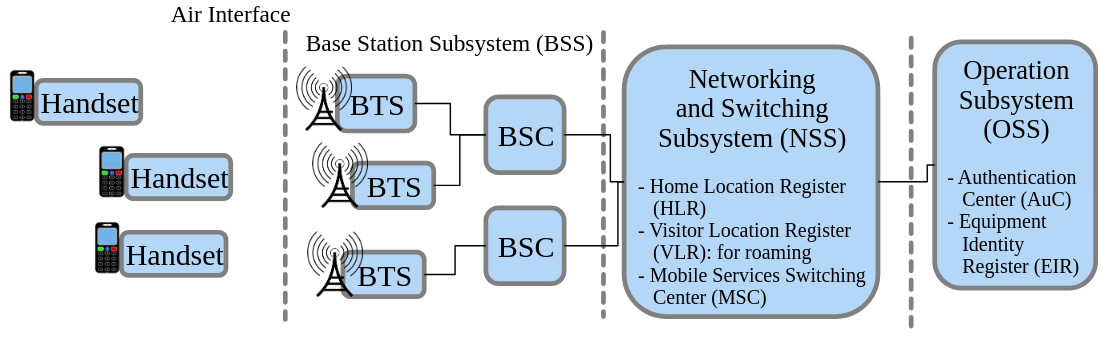
\includegraphics[width=0.9\columnwidth]{Resources/gsm.png}\\
BTS: Base Tranceiver Station\\
BSC: Base Station Controller\\
\begin{itemize}
  \item Circuit-switched network, designed for voice communication
    \begin{itemize}
      \item Stable channel between communication partners is reserved
      \item Seperate channel for signaling (different time slices)
      \item Slow, expensive
      \item GSM introduces SMS: small texts can be transferred in signaling channel
    \end{itemize}
\end{itemize}

\subsubsection{Secuirty}
\begin{itemize}
  \item Goal: "At least as secure as a landline"
  \item Security functions
    \begin{itemize}
      \item Autentication and Key Agreement (AKA)
        \begin{itemize}
          \item Shared secren in AuC and SIM
          \item Authentication via challange-response protocol
          \item "Agreement" on short term session keys for encryption
        \end{itemize}
      \item Confidentiality Protection
        \begin{itemize}
          \item Encryption of user data ("user plane")
          \item Encryption of signalling ("control plane")
        \end{itemize}
      \item Integrity Protection
        \begin{itemize}
          \item Only for signalling
          \item Often "implicitly" by encryption
        \end{itemize}
    \end{itemize}
\end{itemize}

\subsubsection{(U)SIM}
\begin{itemize}
    \item \textbf{SIM card} introduced with \textbf{GSM}
    \begin{itemize}
        \item \textbf{SIM:} \emph{Subscriber Identity Module}
        \item \textbf{International mobile subscriber identity (IMSI)}
        \begin{itemize}
            \item \emph{Temporary mobile subscriber identity (TMSI):} derived from IMSI
        \end{itemize}
        \item \textbf{Security token (smartcard)} of the network operator
        \begin{itemize}
            \item Typically implemented on a JavaCard
            \item Identifies the network subscriber (\emph{“customer”} of the \textbf{MNO})
            \item Subscriber key \(K_i\) (128 bit)
        \end{itemize}
        \item \textbf{Standardized crypto} \(\Rightarrow\) roaming possible
        \item Independent from mobile equipment (\textbf{ME})
        \begin{itemize}
            \item \textbf{International Mobile Equipment Identifier (IMEI)} identifies the device
            \item SIM can be used with any \textbf{ME} (but: SIM-Lock prevents changing SIM for some devices)
        \end{itemize}
    \end{itemize}
    \item \textbf{USIM: Universal SIM} \(\rightarrow\) \textbf{UMTS} (typically implemented in UICC, together with (GSM-) SIM)
\end{itemize}

\subsubsection{Crypto Algorithms}
\begin{itemize}
    \item \textbf{Authentication: A3}
    \begin{itemize}
        \item \emph{Variants: COMP128 (broken)}
        \item \emph{Later: COMP128-2 (only 54 key bits), COMP128-3 (64 key bits), COMP128-4}
    \end{itemize}

    \item \textbf{Key Generation: A8}
    \begin{itemize}
        \item \emph{Variants: COMP128, COMP128-2, COMP128-3, COMP128-4}
    \end{itemize}

    \item \textbf{Encryption: A5 (stream cipher)}
    \begin{itemize}
        \item \emph{A5/0 (no encryption), A5/1 (broken), A5/2 (weakened version of A5/1)}
        \item \emph{Later: A5/3 (KASUMI -- also broken)}
    \end{itemize}
\end{itemize}

\subsubsection{Authentication}
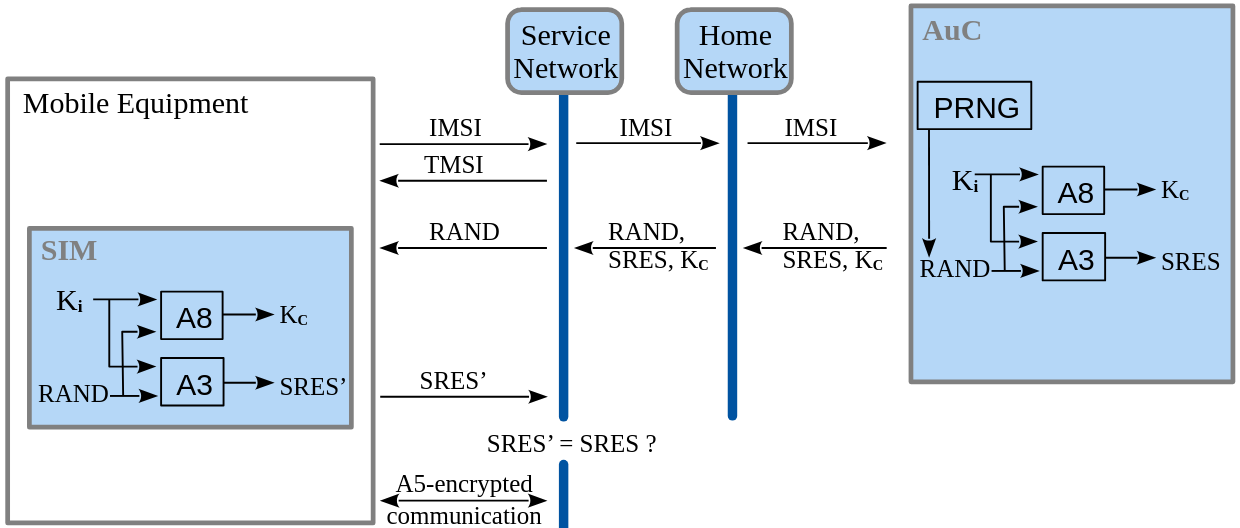
\includegraphics[width=0.9\columnwidth]{Resources/gsm_auth.png} % Adjust width and path
\begin{itemize}
    \item The \textbf{Service Network} sends a \textbf{RAND} (random challenge) to the Mobile Equipment (ME).
    \item The SIM card computes:
    \begin{itemize}
        \item \textbf{SRES'}: The signed response, using the authentication algorithm A3 and the subscriber key (\(K_i\)).
        \item \textbf{\(K_c\)}: The session key for encryption, generated using algorithm A8 and \(K_i\).
    \end{itemize}
    \item The \textbf{Authentication Center (AuC)} in the Home Network performs the same computations (using \(K_i\) stored in its database) to generate \textbf{SRES}.
    \item The network compares the \textbf{SRES'} received from the ME with its own \textbf{SRES}. If they match, authentication is successful.
    \item Communication is encrypted using the generated \textbf{\(K_c\)} and the A5 stream cipher.
\end{itemize}
\textbf{Glossary:}
\begin{itemize}
    \item \textbf{IMSI:} International Mobile Subscriber Identity, a unique identifier for the subscriber.
    \item \textbf{TMSI:} Temporary Mobile Subscriber Identity, a pseudonym for the IMSI used for privacy.
    \item \textbf{\(K_i\):} Subscriber key, stored on the SIM and at the network's Authentication Center.
    \item \textbf{PRNG:} Pseudo-Random Number Generator, used to generate the RAND challenge.
\end{itemize}

\subsubsection{IMSI Catcher}
\begin{itemize}
    \item \textbf{Man-in-the-Middle attack:}
    \begin{itemize}
        \item \textbf{IMSI Catcher:} A device (e.g., “Stingray”) impersonates a legitimate Base Station to intercept communications.
        \item \textbf{Step-by-step process:}
        \begin{itemize}
            \item The IMSI catcher pretends to be a Base Station with a strong signal, forcing nearby mobile devices to connect.
            \item The mobile device sends its IMSI (International Mobile Subscriber Identity) to the catcher for authentication.
            \item The IMSI catcher forwards authentication requests to the real Base Station, acting as a mobile phone.
            \item Once connected, the IMSI catcher can:
            \begin{itemize}
                \item Intercept data and voice traffic.
                \item Disable encryption by negotiating an unencrypted or weaker cipher mode.
                \item Track users by capturing their IMSI or location data.
            \end{itemize}
        \end{itemize}
        \item This method exploits the lack of mutual authentication in GSM networks (i.e., the mobile phone does not verify the Base Station's authenticity).
    \end{itemize}
\end{itemize}

\subsection{UMTS}
\subsubsection{Security Improvements}
\begin{itemize}
    \item \textbf{3GPP} (\emph{3rd Generation Partnership Project})
    \begin{itemize}
        \item Responsible for specifications, including issuing \emph{5G standards}.
    \end{itemize}
    \item \textbf{“Old” GSM SIM cards} can still be used:
    \begin{itemize}
        \item Backwards compatibility supports GSM authentication protocols.
    \end{itemize}
    \item \textbf{Circuit and Packet Switching:} Both methods available for communication.
    \item \textbf{Improved Crypto:}
    \begin{itemize}
        \item \emph{3GPP publishes cryptographic algorithms.}
        \item Encryption is applied \textbf{not only on the air}, enhancing security.
    \end{itemize}
    \item \textbf{New Encryption Algorithms:}
    \begin{itemize}
        \item Initially introduced \textbf{KASUMI}, used for encryption and CBC-MAC.
        \item Later replaced by more secure algorithms, as \textbf{KASUMI was broken}.
    \end{itemize}
    \item \textbf{Mutual Authentication:} 
    \begin{itemize}
        \item \emph{Both user and network authenticate each other (not mandatory).}
    \end{itemize}
    \item \textbf{Main Problems:}
    \begin{itemize}
        \item Backwards compatibility creates vulnerabilities.
        \item \emph{Fallback to GSM weakens overall security.}
    \end{itemize}
\end{itemize}

\subsection{LTE- Long Term Evolution}
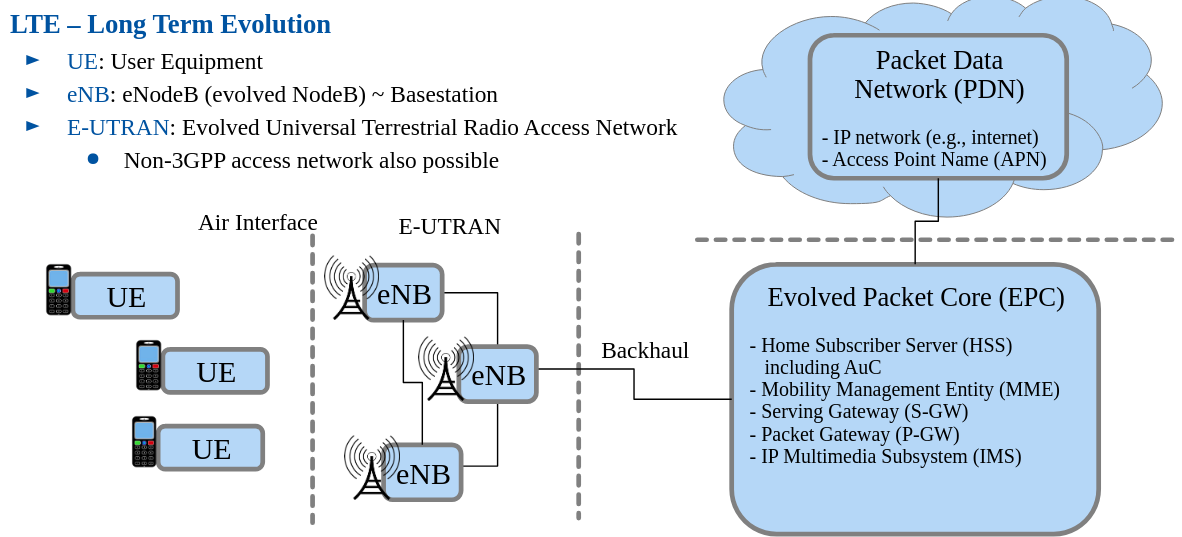
\includegraphics[width=1\columnwidth]{Resources/lte.png}
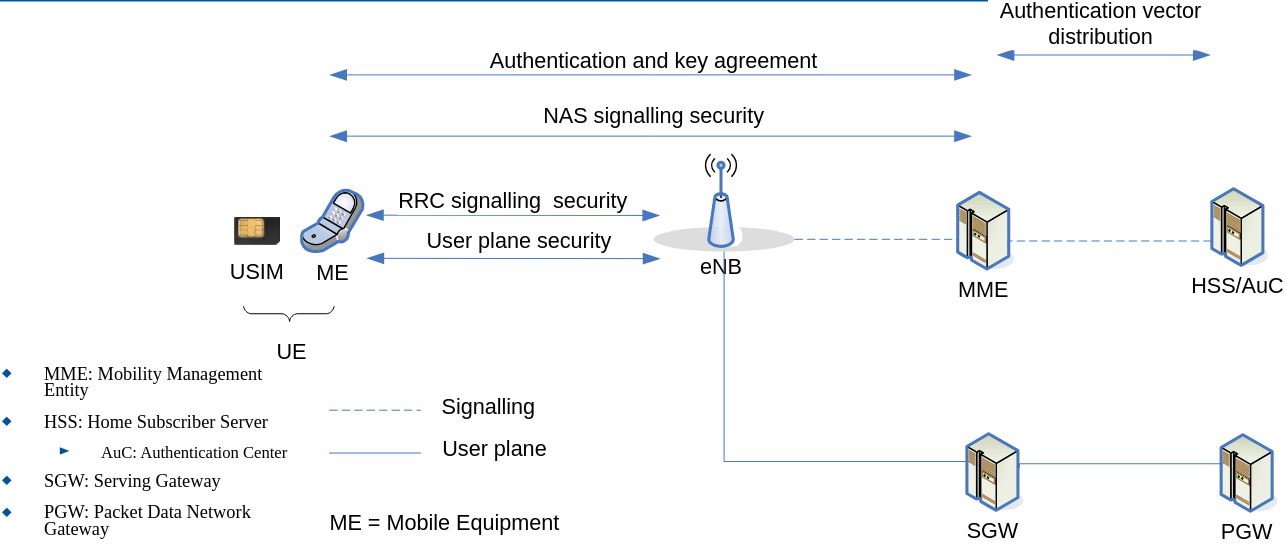
\includegraphics[width=1\columnwidth]{Resources/lte2.png}

\subsubsection{Protocol Stack}
\subsubsection{LTE Protocol Stack}
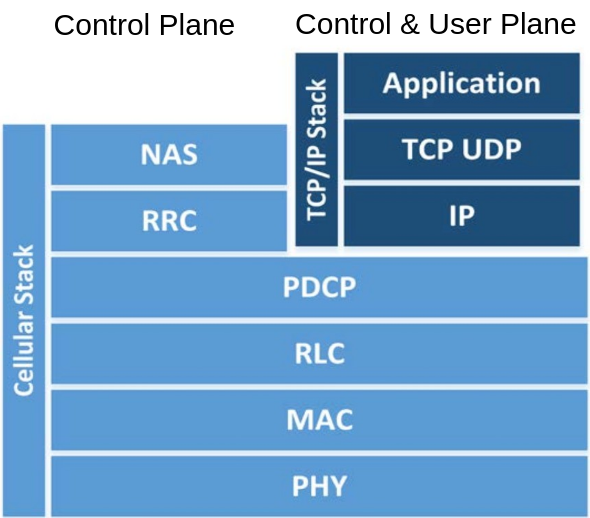
\includegraphics[width=0.3\columnwidth]{Resources/lte_protocols.png} % Adjust width and path
\begin{itemize}
    \item \textbf{Control Plane:}
    \begin{itemize}
        \item Handles signaling, network resource management, and routing.
        \item Ensures communication setup and maintenance.
    \end{itemize}
    \item \textbf{User Plane:}
    \begin{itemize}
        \item Responsible for transferring user data (e.g., voice, video, and application data).
        \item Integrates directly with applications via the TCP/IP stack.
    \end{itemize}
    \item \textbf{Key Protocols (Cellular Stack):}
    \begin{itemize}
        \item \textbf{NAS (Non-Access Stratum):}
        \begin{itemize}
            \item Manages mobility and session-related signaling between the UE and the core network (e.g., authentication, location updates).
        \end{itemize}
        \item \textbf{RRC (Radio Resource Control):}
        \begin{itemize}
            \item Handles signaling at the radio level, such as connection setup, handovers, and state management.
        \end{itemize}
        \item \textbf{PDCP (Packet Data Convergence Protocol):}
        \begin{itemize}
            \item Provides header compression, encryption, and integrity protection for user and control plane data.
        \end{itemize}
        \item \textbf{RLC (Radio Link Control):}
        \begin{itemize}
            \item Ensures data reliability through retransmissions and error correction.
        \end{itemize}
        \item \textbf{MAC (Medium Access Control):}
        \begin{itemize}
            \item Manages resource allocation and data multiplexing for multiple UEs.
        \end{itemize}
        \item \textbf{PHY (Physical Layer):}
        \begin{itemize}
            \item Deals with the actual transmission of radio signals over the air interface.
        \end{itemize}
    \end{itemize}
    \item \textbf{Integration with Applications:}
    \begin{itemize}
        \item The LTE stack works alongside the TCP/IP stack for application-level data transfer:
        \begin{itemize}
            \item Application protocols (e.g., HTTP, VoIP) run on top of \textbf{TCP/UDP}.
            \item \textbf{IP} ensures routing and addressing across networks.
            \item PDCP compresses and encrypts packets before passing them to the lower layers for radio transmission.
        \end{itemize}
    \end{itemize}
\end{itemize}
\subsubsection{Authentication}
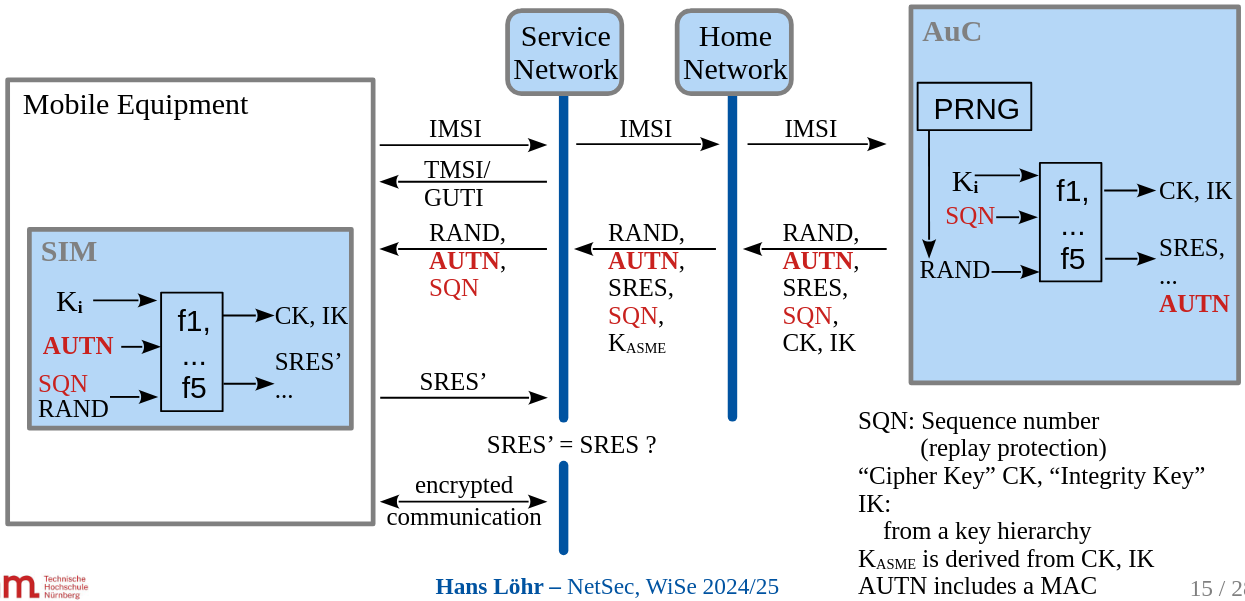
\includegraphics[width=0.8\columnwidth]{Resources/lte_auth.png} 
\begin{itemize}
    \item \textbf{Authentication Process:}
    \begin{itemize}
        \item The \textbf{Home Network} sends a random challenge (\textbf{RAND}), an authentication token (\textbf{AUTN}), and a sequence number (\textbf{SQN}) to the \textbf{Mobile Equipment (ME)}.
        \item The \textbf{SIM card} in the ME uses the \textbf{subscriber key (\(K_i\))} and predefined functions (\(f1, f2, \ldots, f5\)) to compute:
        \begin{itemize}
            \item \textbf{SRES':} Signed response for authentication.
            \item \textbf{CK:} Cipher key for encryption.
            \item \textbf{IK:} Integrity key for data integrity.
        \end{itemize}
        \item The \textbf{ME} sends \textbf{SRES'} back to the network for verification.
        \item If \textbf{SRES'} matches the expected \textbf{SRES}, authentication is successful, and encrypted communication begins.
    \end{itemize}

    \item \textbf{Acronyms:}
    \begin{itemize}
        \item \textbf{RAND:} Random number used for the challenge.
        \item \textbf{AUTN:} Authentication token, includes a MAC (Message Authentication Code).
        \item \textbf{SQN:} Sequence number for replay protection.
        \item \textbf{\(K_i\):} Subscriber key shared between SIM and the Home Network.
        \item \textbf{CK:} Cipher key, used for encrypting data.
        \item \textbf{IK:} Integrity key, used for ensuring data integrity.
        \item \textbf{K\(_{\text{ASME}}\):} Key derived from \textbf{CK} and \textbf{IK}, used for session management.
    \end{itemize}

    \item \textbf{Security Features:}
    \begin{itemize}
        \item Protects against replay attacks using \textbf{SQN}.
        \item Ensures mutual authentication with \textbf{AUTN} and \textbf{SRES}.
        \item Enables encrypted communication using \textbf{CK}.
    \end{itemize}
\end{itemize}

\subsubsection{Crypto Algorithms}
\begin{itemize}
    \item \textbf{Authentication Algorithms:}
    \begin{itemize}
        \item \(f1, f2\): Message Authentication Codes (MACs), inherited from UMTS.
        \item Operator-specific (\textbf{MNO-dependent}); 3GPP recommends AES-based algorithms.
    \end{itemize}

    \item \textbf{Key Generation Algorithms (Key Derivation):}
    \begin{itemize}
        \item \(f3, f4, f5\): Used for deriving keys (e.g., \(K_c, K_i\)), also inherited from UMTS.
        \item Operator-specific (\textbf{MNO-dependent}); 3GPP recommends AES-based algorithms.
    \end{itemize}

    \item \textbf{Encryption Algorithms:}
    \begin{itemize}
        \item \textbf{EEA0:} "Null cipher" (no encryption).
        \item \textbf{128-EEA1:} SNOW 3G (stream cipher).
        \item \textbf{128-EEA2:} AES-based encryption algorithm (strong and widely used).
        \item \textbf{128-EEA3:} ZUC (Chinese stream cipher).
    \end{itemize}

    \item \textbf{Integrity Algorithms (EIA):}
    \begin{itemize}
        \item Similar to encryption, used to ensure data integrity during transmission.
    \end{itemize}
\end{itemize}

\subsubsection{Privacy}
\begin{itemize}
    \item \textbf{Fact:} Mobile Network Operators (MNOs) can always track their users (this is by design).
    \item \textbf{Additional Problem:} Eavesdropping on radio communication.
    \begin{itemize}
        \item \textbf{IMSI:} A unique identifier for a user:
        \begin{itemize}
            \item \textbf{GSM:} Used by the UE only when no \textbf{TMSI} is available.
            \item \textbf{LTE:} \textbf{IMSI} replaced by \textbf{GUTI} (Globally Unique Temporary Identifier).
        \end{itemize}
        \item \textbf{TMSI/GUTI}:
        \begin{itemize}
            \item Can (and should) be \textbf{updated frequently} to avoid tracking by third parties.
            \item Changes must be \textbf{unpredictable} to prevent tracking or identification.
        \end{itemize}
        \item Research findings:
        \begin{itemize}
            \item 19 out of 28 MNOs used \textbf{very simple, predictable patterns}, such as monotonic counters.
            \item Earlier research found \textbf{no or very rare changes}, allowing tracking.
        \end{itemize}
    \end{itemize}
\end{itemize}

\subsubsection{LTE Proximity Services (ProSe)}
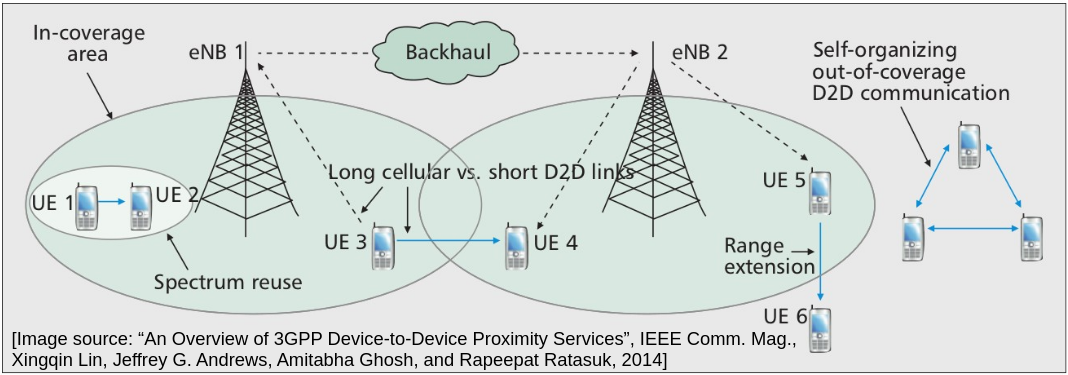
\includegraphics[width=0.7\columnwidth]{Resources/prose.png} 
\begin{itemize}
    \item \textbf{ProSe:} Cellular Device-to-Device (D2D) Communication
    \begin{itemize}
        \item Enables communication between devices directly, bypassing base stations.
        \item Can operate \textbf{with or without network coverage.}
        \item Commonly used in \textbf{public safety networks}, such as emergencies or disasters.
        \item \textbf{Applications:}
        \begin{itemize}
            \item Peer-to-peer applications.
            \item Location-based services.
            \item Range extension through device relays.
        \end{itemize}
    \end{itemize}

    \item \textbf{Control Modes:}\\
    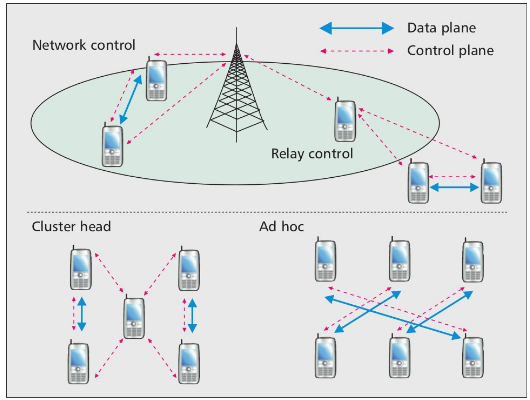
\includegraphics[width=0.5\columnwidth]{Resources/prose2.png} 
    \begin{itemize}
        \item \textbf{Network-Controlled Mode:}
        \begin{itemize}
            \item ProSe communication is managed via the LTE network for reliability and resource allocation.
        \end{itemize}
        \item \textbf{Cluster Head Mode:}
        \begin{itemize}
            \item A device (cluster head) acts as a local coordinator for nearby devices.
            \item Manages intra-cluster communication and relays data to the LTE network or other clusters.
        \end{itemize}
        \item \textbf{Ad Hoc Mode:}
        \begin{itemize}
            \item Devices communicate directly without centralized control.
            \item Suitable for completely out-of-coverage scenarios.
        \end{itemize}
    \end{itemize}

    \item \textbf{Key Management:}
    \begin{itemize}
        \item \textbf{Authorization:} User Equipment (UE) must be authorized unless pre-configured on the USIM.
        \item \textbf{MIKEY (Multimedia Internet Keying):}
        \begin{itemize}
            \item Used for VoIP key exchange.
            \item Supports different modes (e.g., pre-shared keys or PKI-based).
        \end{itemize}
        \item \textbf{Key Hierarchy:}
        \begin{itemize}
            \item ProSe MIKEY Key (PMK) → Temporary ProSe Group Key (PGK).
            \item PGK → ProSe Traffic Key (PTK) → ProSe Encryption Key (PEK).
        \end{itemize}
    \end{itemize}
\end{itemize}

\subsection{5G: The 5\textsuperscript{th} Generation Mobile Network}
\begin{itemize}
    \item \textbf{5G:} Represents the next and current generation of mobile networks.
    \item \textbf{Deployment:} Has already started, though some specifications are still evolving.
    \item \textbf{Performance:} 
    \begin{itemize}
        \item Much faster than 4G.
        \item Provides significantly lower latency and higher reliability.
    \end{itemize}
    \item \textbf{Advancements:}
    \begin{itemize}
        \item Builds on software-defined networking principles, initiated with LTE.
        \item Includes advanced \textbf{Quality-of-Service (QoS)} features.
    \end{itemize}
    \item \textbf{New Application Scenarios:}
    \begin{itemize}
        \item \textbf{Industry 4.0:} Automation and IoT for manufacturing and logistics.
        \item \textbf{Device-to-Device Communication:} Key for vehicular networks and ProSe.
        \item \textbf{Private Networks:} Operated by non-traditional operators, such as manufacturing industries.
    \end{itemize}
\end{itemize}

\subsubsection{5G Security: Relevant Entities (Functions)}
\begin{itemize}
    \item \textbf{AMF (Access and Mobility Management Function):} 
    Manages device access and mobility in the Serving Network.

    \item \textbf{SEAF (Security Anchor Functionality):} 
    Handles initial authentication and acts as the anchor point for security in the Serving Network.

    \item \textbf{AUSF (Authentication Server Function):} 
    Processes authentication in the Home Network, replacing the HSS from LTE.

    \item \textbf{ARPF (Authentication Credential Repository and Processing Function):} 
    Stores and processes authentication keys, like the AuC in LTE.

    \item \textbf{SEPP (Security Edge Protection Proxy):} 
    Secures inter-operator communication (e.g., roaming) by protecting signaling messages exchanged between networks.\\
    \\
\end{itemize}
\begin{itemize}
    \item \textbf{IMSI → SUPI (Subscription Permanent Identifier):}
    \begin{itemize}
        \item \textbf{SUPI:} Replaces IMSI and is never transmitted unencrypted over the air.
        \item \textbf{SUCI (Subscription Concealed Identifier):}
        \begin{itemize}
            \item SUPI is encrypted using the network's public key to create SUCI for secure transmission.
        \end{itemize}
        \item \textbf{TMSI → 5G-S-TMSI:} Mandatory to change after paging (e.g., during basestation handover).
        \item \textbf{GUTI → 5G-GUTI:} Requirements for dynamic GUTI changes to improve privacy.
    \end{itemize}

    \item \textbf{Authentication (AKA):}
    \begin{itemize}
        \item Protocol improvements to better protect security features and enhance user privacy.
    \end{itemize}

    \item \textbf{IMSI Catcher Detection:}
    \begin{itemize}
        \item \textbf{Measurement Reports:} Enable network-based and UE-assisted detection.
        \item Makes IMSI/SUCI catchers harder to deploy without being detected.
    \end{itemize}

    \item \textbf{Security in 5G Standalone Mode:}
    \begin{itemize}
        \item Many advanced features are available only in 5G "Standalone" mode.
        \item Current usage is mainly \textbf{5G NSA (Non-Standalone)} for cooperation with 4G (LTE).
    \end{itemize}
\end{itemize}

\subsubsection{Authentication and Key Agreement}
\begin{itemize}
    \item \textbf{Authentication Options:}
    \begin{itemize}
        \item \textbf{EAP-AKA'}:
        \begin{itemize}
            \item Defined in RFC5448.
            \item Based on pre-shared keys.
            \item Fits into the EAP (Extensible Authentication Protocol) framework.
        \end{itemize}
        \item \textbf{5G AKA}:
        \begin{itemize}
            \item Derived from LTE AKA for backward compatibility.
        \end{itemize}
    \end{itemize}

    \item \textbf{Privacy Concerns:}
    \begin{itemize}
        \item Flaws in 5G AKA found via formal protocol analysis:
        \begin{itemize}
            \item \textit{David Basin et al., "A Formal Analysis of 5G Authentication", ACM CCS 2018}.
        \end{itemize}
        \item Practical attacks require targeting specific users:
        \begin{itemize}
            \item \textit{Chlosta, Rupprecht, Pöpper, Holz, "5G SUCI-Catchers: Still catching them all?", ACM WiSec 2021}.
        \end{itemize}
    \end{itemize}
\end{itemize}

\subsubsection{Service-Based Interfaces}
\begin{itemize}
    \item \textbf{Network Operators and 3rd Parties Offering "Services":}
    \begin{itemize}
        \item \textbf{Network Functions (NF):} Core network features exposed as services.
        \item \textbf{Other Services:} Additional functionalities provided by the network.
        \item \textbf{TLS Support:} Ensures secure communication between entities.
        \item \textbf{OAuth 2.0-based Authorization:} Allows secure access control using access tokens.
    \end{itemize}

    \item \textbf{Network Slices:}
    \begin{itemize}
        \item Provides virtualized and isolated network partitions with specific \textbf{QoS (Quality of Service)} properties.
        \item Uses \textbf{EAP-based Authorization} for access control.
    \end{itemize}
\end{itemize}

\section{Firewalls, Intrusion Detection and Prevention}
\subsection{Firewalls}
\begin{itemize}
  \item Firewalls separate networks
    \begin{itemize}
      \item Restricts traffic: enforces policy
      \item Logging
      \item Implemented in SW and/or HW)
    \end{itemize}
\end{itemize}

\subsubsection{Packet Filtering}
\begin{itemize}
    \item \textbf{Packet filtering firewalls:}
    \begin{itemize}
        \item Policies defined by filtering rules (source, destination, port, protocol, etc.).
        \item Rules decide actions: accept, block, log, or modify packets.
        \item Advanced filters can modify packets (e.g., NAT or port translation).
    \end{itemize}

    \item \textbf{Advantages:}
    \begin{itemize}
        \item Cheap, widely available, and efficient.
        \item Examples: Linux \texttt{netfilter}, Windows firewall.
        \item Simple implementation; no modification to applications required.
    \end{itemize}

    \item \textbf{Limitations:}
    \begin{itemize}
        \item Susceptible to IP and port spoofing attacks.
        \item Rules limited to individual packets and lack comprehensive state awareness.
        \item Cannot enforce application-specific filtering; lacks deeper protocol knowledge.
        \item Usually not capable of rejecting specific packets within a particular application session.
    \end{itemize}

    \item \textbf{Niche Aspects:}
    \begin{itemize}
        \item Filters can reject IP spoofing by blocking packets from internal addresses arriving at external interfaces.
        \item Access control by ports can restrict services to specific source addresses (e.g., SMTP limited to internal IPs).
        \item Can filter based on packet type (TCP, UDP) or flags (e.g., SYN for connection establishment).
    \end{itemize}
\end{itemize}

\subsubsection{Connection Tracking and Stateful Firewalls}
\begin{itemize}
    \item \textbf{Connection Tracking:}
    \begin{itemize}
        \item Tracks packets belonging to the same logical "connection" (not limited to TCP).
        \item Examples:
        \begin{itemize}
            \item UDP-based connections (e.g., DTLS).
            \item DNS requests/responses and ICMP echo/replies.
        \end{itemize}
        \item Supports protocols with separate control and data connections (e.g., active FTP).
        \item Enables NAT functionality by rewriting addresses for complex protocols.
    \end{itemize}
    
    \item \textbf{Stateful Firewalls:}
    \begin{itemize}
        \item Maintain state information about active connections.
        \item Rules can dynamically adapt based on connection states (e.g., allow replies to outgoing requests).
    \end{itemize}
\end{itemize}

\subsubsection{Linux Firewall: Netfilter}
Netfilter, part of the Linux kernel, is a framework for packet filtering and network address translation (NAT). It operates using a series of hooks in the network stack where rules, organized into \textbf{tables} and \textbf{chains}, are applied.
\paragraph{Chains and Their Functions:}
\begin{itemize}
    \item \textbf{Input Chain:} Handles packets destined for the local system (e.g., filtering SSH traffic).
    \item \textbf{Output Chain:} Manages packets generated locally and leaving the system (e.g., limiting outgoing ICMP traffic).
    \item \textbf{Forward Chain:} Processes packets passing through the system but not destined for it (e.g., traffic routing in a gateway).
    \item \textbf{Prerouting Chain:} Alters incoming packets before routing decisions (e.g., DNAT for port redirection).
    \item \textbf{Postrouting Chain:} Alters outgoing packets after routing decisions (e.g., SNAT for source IP modification).
\end{itemize}
\paragraph{Key Components:}
\begin{itemize}
    \item \textbf{Tables:} Contain chains for specific tasks:
    \begin{itemize}
        \item \textbf{Filter Table:} Default table for packet filtering (Input, Output, Forward chains).
        \item \textbf{NAT Table:} Used for network address translation (Prerouting, Postrouting chains).
        \item \textbf{Mangle Table:} For modifying packet headers.
    \end{itemize}
    \item \textbf{Tools:}
    \begin{itemize}
        \item \texttt{iptables}: Legacy tool for managing rules.
        \item \texttt{nftables}: Modern replacement offering simplified syntax and better performance.
    \end{itemize}
\end{itemize}
\paragraph{Use Case Example:}
A packet enters the system through the \textbf{Prerouting Chain}, is routed to the appropriate interface (via \textbf{Forward Chain} if being forwarded or \textbf{Input Chain} if destined locally), and exits through the \textbf{Postrouting Chain} after necessary modifications.
Netfilter’s modularity and flexibility make it a powerful tool for managing network traffic.

\subsubsection{Application-Level Gateways}
An \textbf{Application-Level Gateway (ALG)} acts as an intermediary between clients and applications, offering fine-grained control and monitoring of traffic specific to application protocols. It provides a specialized interface tailored for applications, such as SMTP or HTTP, allowing for filtering, logging, and user profiling at the application layer.
\paragraph{Functionality:}
\begin{itemize}
    \item \textbf{Connection Handling:} Clients connect to the gateway, which filters and analyzes the traffic before forwarding it to the application server.
    \item \textbf{Protocol Awareness:} Equipped with detailed knowledge of application-specific protocols, enabling in-depth traffic inspection and filtering.
    \item \textbf{State Management:} Tracks the state of connections or application data to enforce security or logging policies effectively.
\end{itemize}
\begin{itemize}
    \item In-depth analysis and traffic filtering based on application logic.
    \item Enables user profiling, attack detection, and intrusion prevention.
    \item Provides application-specific caching and potential for secure communication.
    \item App extensions for additional features, such as authentication, without modifying the original application.
\end{itemize}
\paragraph{Limitations:}
\begin{itemize}
    \item \textbf{Performance Overhead:} The inspection and filtering process can reduce throughput.
    \item \textbf{Maintenance Effort:} Requires frequent updates to stay compatible with evolving application protocols.
    \item \textbf{Limited Scope:} Only supports predefined applications, limiting flexibility in heterogeneous environments.
\end{itemize}
\paragraph{Use Case:}
ALGs are frequently employed in enterprise environments for managing email servers (e.g., SMTP gateways) or for secure access to critical applications by acting as a filter and logging interface for external traffic.

\subsubsection{Proxy Firewalls}
Proxy firewalls act as a generic proxy on the transport layer, enabling advanced traffic control and enhancing communication security.
\paragraph{Key Features:}
\begin{itemize}
    \item \textbf{Connection State Tracking:} Monitors and manages the state of connections.
    \item \textbf{Authentication and Security:} Adds user authentication and communication security.
    \begin{itemize}
        \item Frequently used in corporate environments:
        \begin{itemize}
            \item Outgoing traffic is routed only via the proxy.
            \item User authentication is required before access.
            \item Only specific ports or applications are allowed.
        \end{itemize}
    \end{itemize}
    \item \textbf{Flexibility:} Can extend functionality toward application-level filtering (e.g., web proxies or caches).
\end{itemize}
\paragraph{Comparison to Application-Level Gateways:}
\begin{itemize}
    \item Proxy firewalls are more general than application-level gateways.
    \item The distinction between proxy firewalls and application gateways is not always clear.
\end{itemize}

\subsubsection*{Firewall Architectures: Dual-Homed Firewall vs. DMZ}
\begin{itemize}
    \item \textbf{Dual-Homed Firewall:}\\
    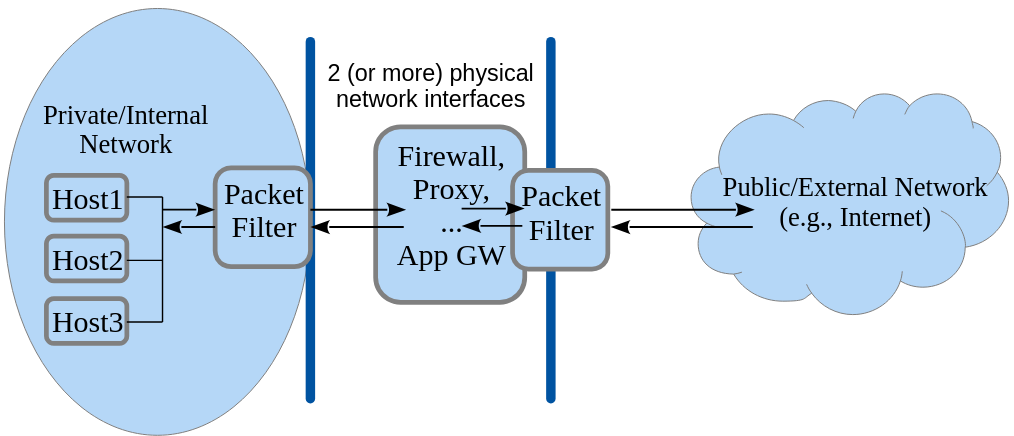
\includegraphics[width=0.7\columnwidth]{Resources/dual-homed.png} 
    \begin{itemize}
        \item \textit{Concept:} Firewall with two interfaces separating internal and external networks.
        \item \textit{Operation:} Traffic flows through the firewall, using packet filters or proxies for mediation.
        \item \textit{Advantages:}
        \begin{itemize}
            \item Strong physical isolation.
            \item Centralized traffic control.
            \item Flexible integration of security mechanisms.
        \end{itemize}
        \item \textit{Disadvantages:}
        \begin{itemize}
            \item Requires additional hardware resources.
            \item Limited scalability for complex networks.
        \end{itemize}
        \item \textit{Use Cases:} Suitable for small/medium networks needing strict isolation.
    \end{itemize}

    \item \textbf{Demilitarized Zone (DMZ):}\\
    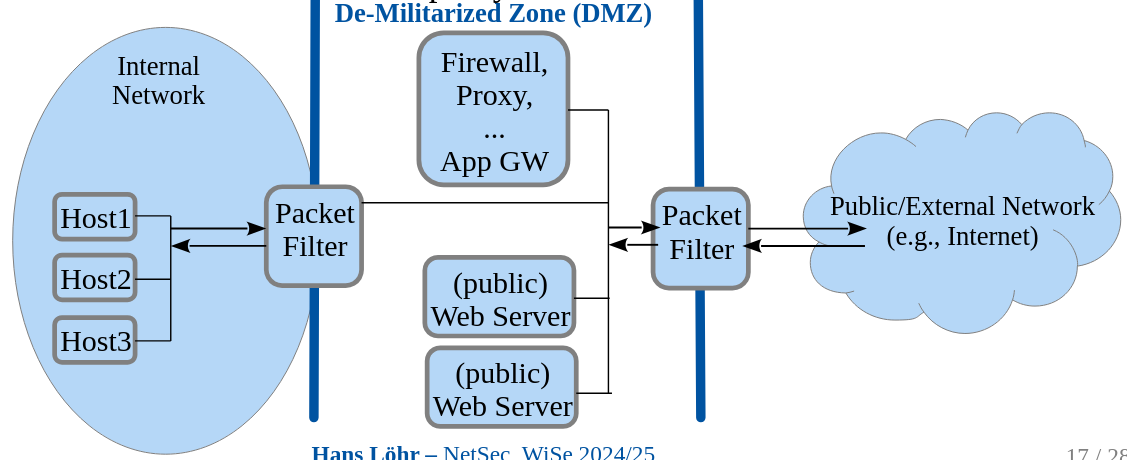
\includegraphics[width=0.8\columnwidth]{Resources/dmz.png} 
    \begin{itemize}
        \item \textit{Concept:} Segregated network zone for public-facing services (e.g., web servers).
        \item \textit{Operation:} Packet filters manage traffic to/from DMZ, preventing direct internal access.
        \item \textit{Advantages:}
        \begin{itemize}
            \item Protects internal networks from compromised public-facing services.
            \item Granular traffic control for specific services.
            \item Limits exposure of internal systems.
        \end{itemize}
        \item \textit{Disadvantages:}
        \begin{itemize}
            \item Adds configuration and maintenance complexity.
        \end{itemize}
        \item \textit{Use Cases:} Ideal for hosting public services (e.g., web hosting, e-commerce).
    \end{itemize}

    \item \textbf{Key Differences:}
    \begin{itemize}
        \item Dual-Homed focuses on isolation, while DMZ separates public services from internal systems.
        \item DMZ adds a dedicated network segment for external-facing servers.
    \end{itemize}
\end{itemize}

\subsection{Intrusion Detection and Prevention System (IDPS)}
\begin{itemize}
    \item \textbf{Intrusion Detection Systems (IDSs):}
    \begin{itemize}
        \item Detect attempts to attack or intrusions.
        \item Focused on monitoring and logging suspicious activities.
    \end{itemize}
    \item \textbf{Prevention:}
    \begin{itemize}
        \item React to detected intrusions to prevent successful attacks.
        \item Goal: Stop attacks in progress by blocking or responding.
    \end{itemize}
    \item \textbf{IDPS = IDS + Prevention:} Combines detection and prevention to ensure proactive and reactive defense mechanisms.
    \item \textbf{Historical Work:}
    \begin{itemize}
        \item James Anderson: \emph{Computer Security Threat Monitoring and Surveillance} (1980).
        \item Dorothy Denning: \emph{An Intrusion Detection Model} (1987).
    \end{itemize}
\end{itemize}
\paragraph{Why Use IDPS?}
\begin{itemize}
    \item Identify incidents effectively.
    \item Support incident response to minimize damage.
    \item Identify gaps in security policy and practices.
    \item Deter insiders from violating policies.
\end{itemize}

\subsubsection{IDPS Functionality (High-Level)}
\begin{itemize}
    \item \textbf{Record Events:}
    \begin{itemize}
        \item Logging and accounting for detected activities.
        \item Observations useful for detecting and analyzing incidents.
        \item Integration with Security Information and Event Management (SIEM) systems.
    \end{itemize}
    \item \textbf{Notify Administrators:}
    \begin{itemize}
        \item Alert administrators to take appropriate action.
    \end{itemize}
    \item \textbf{Produce Reports:}
    \begin{itemize}
        \item Summarize activities and detected threats for analysis.
    \end{itemize}
    \item \textbf{Automated First-Level Reaction:}
    \begin{itemize}
        \item Stop attacks or intrusion attempts automatically.
        \item Dynamically change the security environment, e.g., reconfigure firewalls.
    \end{itemize}
\end{itemize}

\subsubsection{Intrusion Detection Model (Denning, 1987)}
\begin{itemize}
    \item \textbf{Components:}
    \begin{itemize}
        \item \textbf{Subjects:} Entities initiating actions.
        \item \textbf{Objects:} Resources being accessed or affected.
        \item \textbf{Audit Records:} Logs of subject actions for monitoring.
        \item \textbf{Profiles:} Behavioral characterizations based on metrics.
        \item \textbf{Anomaly Records:} Highlight abnormal activities.
        \item \textbf{Activity Rules:} Define responses to anomalies (e.g., profile updates, intrusion reporting).
    \end{itemize}
    \item \textbf{Metrics:}
    \begin{itemize}
        \item Event Counters
        \item Interval Timers
        \item Resource Measures
    \end{itemize}
    \item \textbf{Models:}
    \begin{itemize}
        \item \textbf{Statistical Models:} Identify statistical anomalies.
        \begin{itemize}
            \item Mean and Standard Deviation Model
            \item Multivariate Correlation Model
            \item Markov Process Model
            \item Time Series Model
        \end{itemize}
        \item \textbf{Operational Models:} Compare metrics against predefined thresholds.
        \item \textbf{Modern Approaches:} Incorporate Machine Learning/AI for advanced anomaly detection.
    \end{itemize}
\end{itemize}

\subsubsection{Types of IDPS}
\begin{itemize}
    \item \textbf{Network-Based Intrusion Detection System (NIDS):}
    \begin{itemize}
        \item Monitors and analyzes network traffic.
        \item Often integrated with firewalls (tightly or loosely).
        \item Includes specialized Wireless IDPS for wireless networks.
        \item Incorporates Network Behavior Analysis (NBA) for deeper traffic insights.
    \end{itemize}
    \item \textbf{Host-Based Intrusion Detection System (HIDS):}
    \begin{itemize}
        \item Monitors activity on a specific host (server or end-user device).
        \item Analyzes system and application logs, network activity, running processes, and system calls.
        \item Tracks file accesses and configuration changes for anomaly detection.
    \end{itemize}
\end{itemize}

\subsubsection{IDPS Architecture}
\begin{itemize}
    \item \textbf{Sensors (Agents):} Monitor and analyze activity.
    \item \textbf{IDPS Management Server:} Collects information from sensors and manages them.
    \item \textbf{Database:} Serves as a repository for audit records.
    \item \textbf{Admin Console:} Provides a user interface for administrators.
\end{itemize}

\subsubsection{Detection Methodologies: Categorization}
\begin{itemize}
    \item \textbf{Signature-Based Intrusion Detection}
    \begin{itemize}
        \item Uses fixed patterns to identify \textit{known threats} (e.g., hash values of malware).
        \item Limited to known threats and can be evaded by intelligent attackers.
    \end{itemize}
    \item \textbf{Anomaly-Based Intrusion Detection}
    \begin{itemize}
        \item Detects previously unknown threats by modeling normal/abnormal behavior.
        \item Requires a \textit{training/learning phase} for data collection and profiling.
        \item Often uses Machine Learning or AI; main focus of current research.
    \end{itemize}
    \item \textbf{Specification-Based Intrusion Detection (Stateful Protocol Analysis)}
    \begin{itemize}
        \item Compares observations to models/specifications of legitimate behavior.
        \item Can be integrated into application-level gateways.
    \end{itemize}
\end{itemize}

\subsection{Summary}
\begin{itemize}
    \item \textbf{Firewalls}
    \begin{itemize}
        \item Essential building block for network security.
        \item Alone cannot effectively prevent attacks.
        \item Various types:
        \begin{itemize}
            \item Packet filters.
            \item Application-level gateways/proxies.
        \end{itemize}
        \item Example: Linux firewall (netfilter, iptables/nftables).
    \end{itemize}
    \item \textbf{Intrusion Detection and Prevention Systems (IDPS)}
    \begin{itemize}
        \item Detect and prevent intrusion attempts.
        \item Types:
        \begin{itemize}
            \item Host-based vs. Network-based IDPS.
        \end{itemize}
        \item Detection methodologies:
        \begin{itemize}
            \item Signature-based.
            \item Behavior-based (e.g., anomaly detection).
        \end{itemize}
        \item Specialized IDPS for specific systems (e.g., industrial automation, vehicle networks).
    \end{itemize}
\end{itemize}

\section{Border Gateway Protocol (BGP), Domain Name System (DNS)}
